\documentclass{beamer}

\usepackage[british]{babel}
\usepackage{graphicx,hyperref,ru,url}
\usepackage{fontspec}
\usefonttheme[onlymath]{serif}
\usepackage{xeCJK}
\usepackage{indentfirst}
\usepackage{longtable}
\usepackage{graphicx}
\usepackage{float}
\usepackage{rotating}
\usepackage{subfigure}
\usepackage{tabu}
\usepackage{amsmath}
\usepackage{amssymb}
\usepackage{setspace}
\usepackage{amsfonts}
\usepackage{appendix}
\usepackage{listings}
\usepackage{multicol}
 \usepackage{ulem}
\usepackage{xcolor}
\usepackage{geometry}
\setCJKfamilyfont{cjkhwxk}{STXINGKA.TTF}
\newcommand*{\cjkhwxk}{\CJKfamily{cjkhwxk}}
%\newfontfamily{\consolas}{Consolas}
%\newfontfamily{\monaco}{Monaco}
%\setmonofont[Mapping={}]{Consolas}	%英文引号之类的正常显示,相当于设置英文字体
%\setsansfont{Consolas} %设置英文字体 Monaco, Consolas,  Fantasque Sans Mono
%\setmainfont{Times New Roman}
\newfontfamily{\consolas}{YaHeiConsolas.ttf}
\newfontfamily{\monaco}{MONACO.TTF}
\newfontfamily{\ubuntumonoB}{UbuntuMono-B.ttf}
\newfontfamily{\ubuntumonoBI}{UbuntuMono-BI.ttf}
\newfontfamily{\ubuntuR}{Ubuntu-R.ttf}
\newfontfamily{\ubuntuC}{Ubuntu-C.ttf}
\setCJKmainfont{STZHONGS.TTF}
\setmainfont{MONACO.TTF}
\setsansfont{MONACO.TTF}
\setsansfont{UbuntuMono-R.ttf}
%\setsansfont{UbuntuMono-B.ttf}
\newcommand{\verylarge}{\fontsize{60pt}{\baselineskip}\selectfont}  
\newcommand{\chuhao}{\fontsize{44.9pt}{\baselineskip}\selectfont}  
\newcommand{\xiaochu}{\fontsize{38.5pt}{\baselineskip}\selectfont}  
\newcommand{\yihao}{\fontsize{27.8pt}{\baselineskip}\selectfont}  
\newcommand{\xiaoyi}{\fontsize{25.7pt}{\baselineskip}\selectfont}  
\newcommand{\erhao}{\fontsize{23.5pt}{\baselineskip}\selectfont}  
\newcommand{\xiaoerhao}{\fontsize{19.3pt}{\baselineskip}\selectfont} 
\newcommand{\sihao}{\fontsize{14pt}{\baselineskip}\selectfont}      % 字号设置  
\newcommand{\xiaosihao}{\fontsize{12pt}{\baselineskip}\selectfont}  % 字号设置  
\newcommand{\wuhao}{\fontsize{10.5pt}{\baselineskip}\selectfont}    % 字号设置  
\newcommand{\xiaowuhao}{\fontsize{9pt}{\baselineskip}\selectfont}   % 字号设置  
\newcommand{\liuhao}{\fontsize{7.875pt}{\baselineskip}\selectfont}  % 字号设置  
\newcommand{\qihao}{\fontsize{5.25pt}{\baselineskip}\selectfont}    % 字号设置 

\definecolor{cred}{rgb}{0.8,0.8,0.8}
\definecolor{cgreen}{rgb}{0,0.3,0}
\definecolor{cpurple}{rgb}{0.5,0,0.35}
\definecolor{cdocblue}{rgb}{0,0,0.3}
\definecolor{cdark}{rgb}{0.95,1.0,1.0}
\lstset{
	numbers=left,
	numberstyle=\tiny\color{black},
	showspaces=false,
	showstringspaces=false,
	basicstyle={\footnotesize}\consolas\itshape,
	keywordstyle=\color{red}\bfseries,
	commentstyle=\color{cgreen},
	stringstyle=\color{cred},
	frame=lines,
	escapeinside=``,
	xleftmargin=1em,
	xrightmargin=1em, 
	%backgroundcolor=\color{cdark},
	aboveskip=1em,
	breaklines=true,
	tabsize=4
} 

% The title of the presentation:
%  - first a short version which is visible at the bottom of each slide;
%  - second the full title shown on the title slide;
\title[系统科学与工程讨论课]{
  \erhao 关于涌现}

% Optional: a subtitle to be dispalyed on the title slide
%\subtitle{Show where you're from}

% The author(s) of the presentation:
%  - again first a short version to be displayed at the bottom;
%  - next the full list of authors, which may include contact information;
\author[***]{
  ***{ }**********}

% The institute:
%  - to start the name of the university as displayed on the top of each slide
%    this can be adjusted such that you can also create a Dutch version
%  - next the institute information as displayed on the title slide
\institute[\yihao\fontspec{LHANDW.TTF}ACEE]{\sihao {数学科学学院统计学}}

% Add a date and possibly the name of the event to the slides
%  - again first a short version to be shown at the bottom of each slide
%  - second the full date and event name for the title slide
\date[\today]{
  \today \\
  }
\graphicspath{{img/}}
\begin{document}

\begin{frame}
  \titlepage
\end{frame}

\begin{frame}{一棵开花的树}
	\begin{columns}
		\column{0.5\textwidth}<1->
		\begin{figure}[H]
			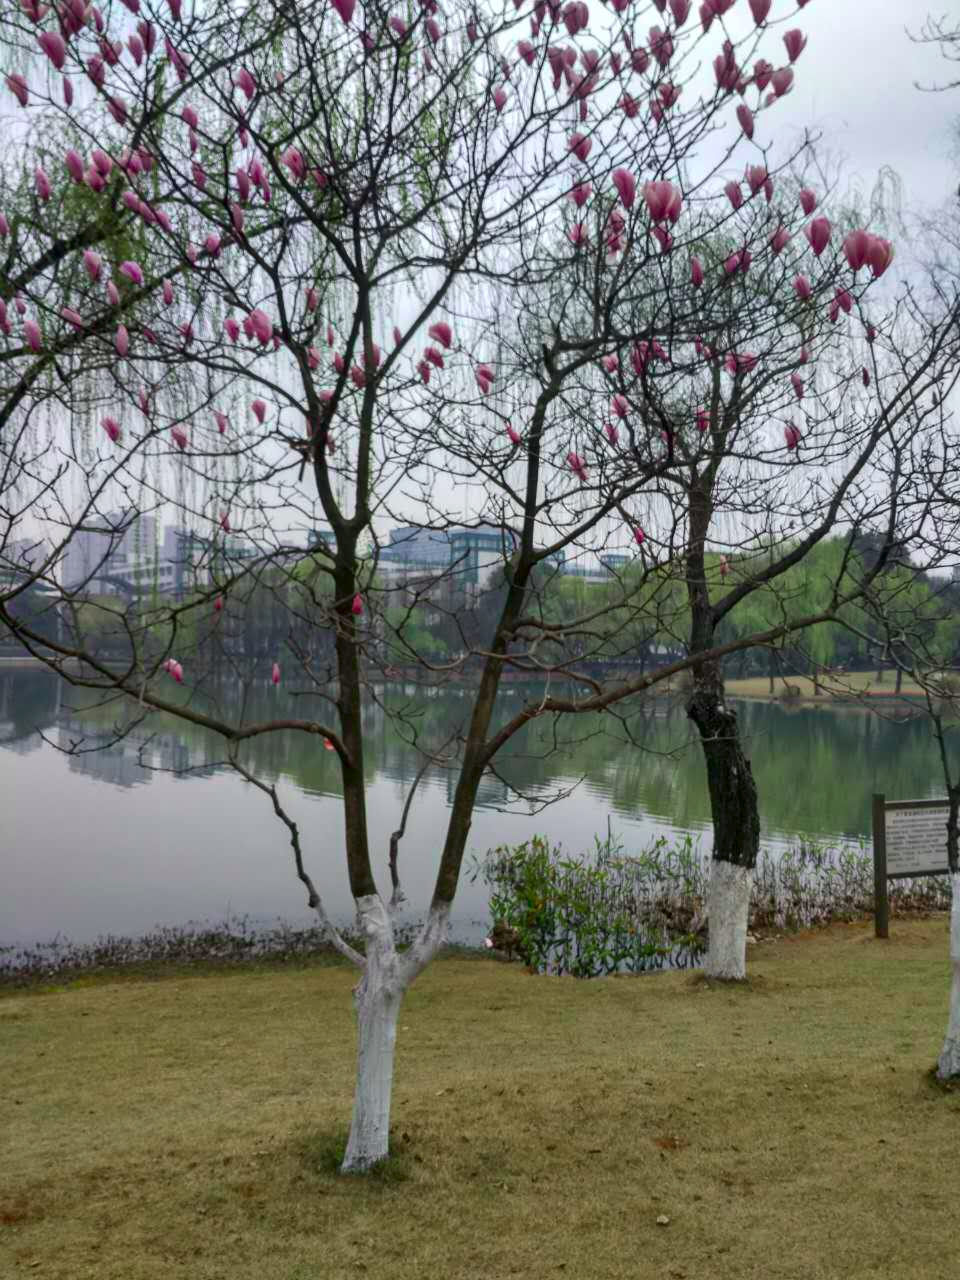
\includegraphics[width=0.85\textwidth]{tree.png}
		\end{figure}
		\column{0.5\textwidth}<2->
	\sout{我已在佛前 求了五百年,\\
	求它让我们结一段尘缘。\\
	佛于是把我化做一棵树,\\
	长在你必经的路旁。\\
	阳光下,\\
	慎重地开满了花,\\
	朵朵都是我前世的盼望!}
	\end{columns}
\end{frame}

\begin{frame}{一棵开花的树}
	\begin{columns}
		\column{0.5\textwidth}
			\begin{figure}[H]
				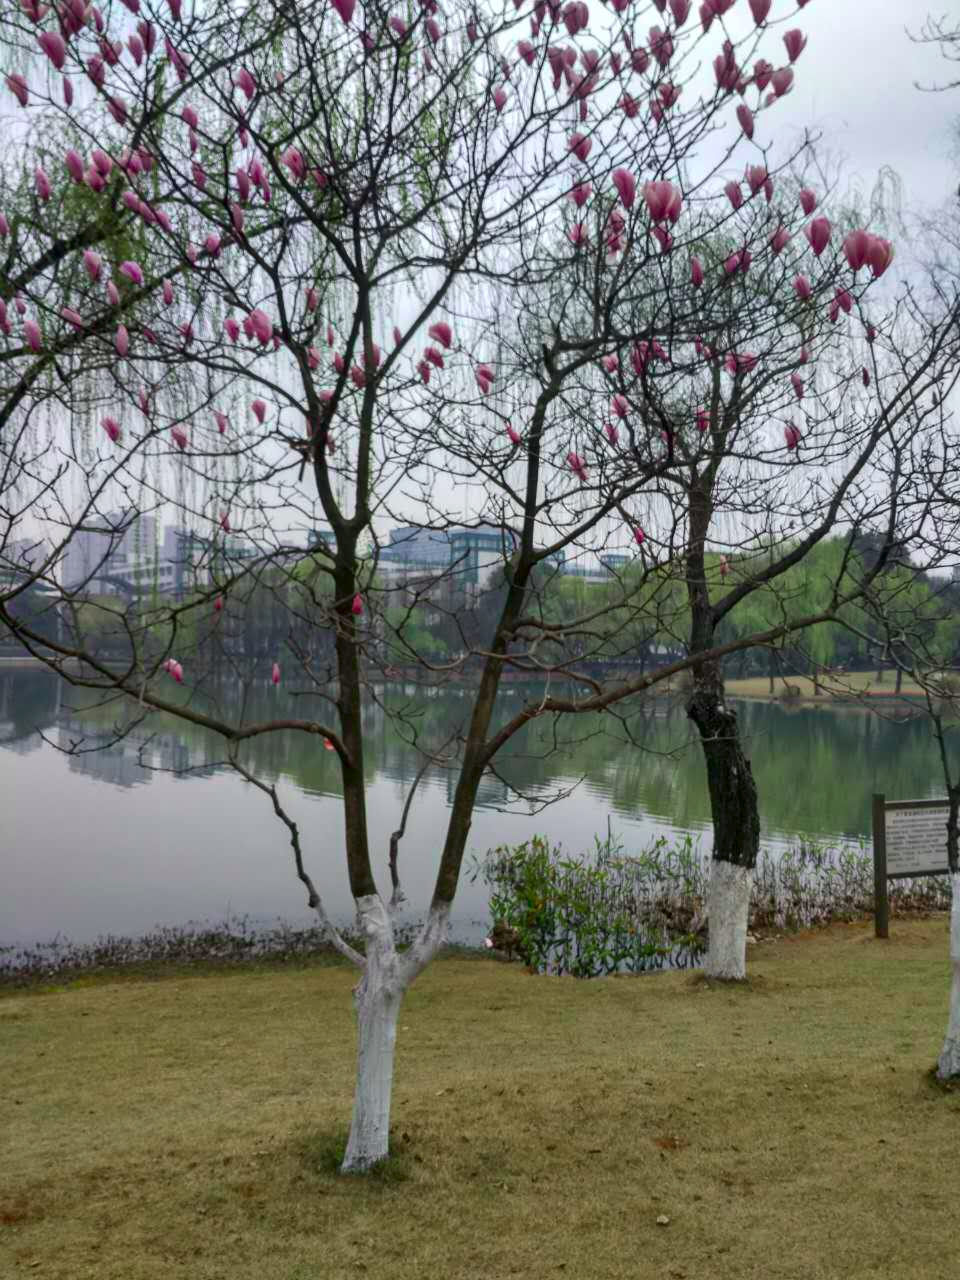
\includegraphics[width=0.85\textwidth]{tree.png}
				\end{figure}
		\column{0.5\textwidth}
		若干年前
		
		一粒种子种到地下
		
		慢慢地变成了一棵会开花的树
	\end{columns}
\end{frame}

\begin{frame}
  \frametitle{内容概要}

  \tableofcontents
\end{frame}

% Section titles are shown in at the top of the slides with the current section 
% highlighted. Note that the number of sections determines the size of the top 
% bar, and hence the university name and logo. If you do not add any sections 
% they will not be visible.
\section{定义}

\begin{frame}{定义}
	\begin{block}{涌现(emergence)}
涌现是一种大的实体通过较小的或较简单的实体间的相互作用而产生的现象,并且大的实体具有小的实体没有的性质。(来自维基百科)
	\end{block}
	\begin{block}{起源}<2->
		亚里士多德的时代已经出现涌现的想法, 这个术语emergent是哲学家G. H. Lewes创造的。
	\end{block}
\end{frame}
\begin{frame}{定义}
	\begin{block}{G. H. Lewes的定义}
		\begin{itemize}
			\item<2-> 每个结果要么是共同作用力量的和,要么是它们的差。
			\begin{itemize}
				\item 当它们方向相同时,为和;
				\item 当方向相反时,为差。
			\end{itemize}
			\item<3-> 否则,是涌现。
			\begin{itemize}
				\item 不是可测量的动作加到可测量的动作上面
				\item 也不是一种类型的事物加到同类型事物上面
				\item 共同作用不相同,因为这些是不可比较的
				\item 结果不是共同作用的和或它们的差。
			\end{itemize}
		\end{itemize}
	\end{block}
\end{frame}
\begin{frame}{定义}
	\begin{block}{弱涌现}
		\begin{itemize}
			\item 由于在元素水平上的相互作用而在系统中产生的新性质
			\item 可以通过观察或模拟系统来确定性质
		\end{itemize}
	\end{block}
	\begin{block}{强涌现}<2->
		\begin{itemize}
			\item 高级系统对其组分的直接因果作用
			\item 以这种方式产生的性质不可能归因于系统的组成部分
			\item 比如,水。
		\end{itemize}
	\end{block}
\end{frame}
\section{性质}
\begin{frame}{性质}
	\begin{block}{性质(Jeffrey Goldstein)}
		\begin{itemize}
		\item 全新的(以前在系统中未观察到的特征)
		\item 一致性或相关性(一段时间内保持自身的综合性整体)
		\item 宏观``水平"(有一些“整体性”的性质)
		\item 它是动力过程的产物(演变)
		\item ``清晰可见的"(可以被感知)
				\end{itemize}
	\end{block}
\end{frame}
\section{发展}
\begin{frame}{发展}
	\begin{block}{还原理论}
		\begin{itemize}
			\item 整体是由局部组成的
			\item 局部决定整体
			\item 整体的任何一个变化都可以在局部找到其原因
			\item 遇到复杂系统的时候会产生一些无法解释的现象,比如生态、人脑、经济系统
		\end{itemize}
	\end{block}
\end{frame}
\begin{frame}{发展}
	\begin{block}{复杂性科学}
		\begin{itemize}
			\item 圣塔菲研究所
			\begin{itemize}
				\item 夸克之父盖尔曼
				\item 经济诺贝尔奖得主阿罗
				\item 遗传算法之父霍兰
			\end{itemize}
			\item 讨论复杂系统中的问题 
			\item 打破了学科间的界限,用一种全新的,统一的视角来认识生命系统、神经系统、经济系统、计算机系统等等,不再关注每个领域的细节
			\item 这些复杂系统的共性中,``涌现"是一种最引人注目的普遍现象
		\end{itemize}
	\end{block}
	
\end{frame}
\section{例子}
\begin{frame}{例子}
	\begin{block}{蚁群}
		\begin{itemize}
			\item 蚂蚁个体的行为是非常机械的(纯粹反射性地被外界条件所驱动)
			\item 大部分行为,都可以用十几条类似咒语的规则来描述
			\begin{itemize}
				\item 用上颚抓紧物体
				\item 根据群体成员的气味来辨别移动着的物体
				\item 根据嗅觉来发现线索
				\item ......
			\end{itemize}
			\item 蚂蚁在变化的环境中移动时,不停地反复调用这些规则
			\item 一旦遇到规则没有描述到的情况,单个蚂蚁将会非常危险
			\item 如,工蚁在规则没有描述到的某一环境中最多只能存活几个星期
		\end{itemize}
	\end{block}
\end{frame}

\begin{frame}{例子}
	\begin{block}{蚁群}
		\begin{itemize}
			\item {\color{red} 然而},作为一个群体,蚁群所显示出的适应性却大大超过了它的个体成员
			\item 充分地表现出这种群体能力
			\begin{itemize}
				\item 寻找食物
				\item 对付敌人
				\item 躲避水灾
				\item ......
			\end{itemize}
			\item 蚁群能够在相当大的程度上按照有利于群体的方式,来调整它们的周围环境。
			\item 蚁群的生存期一般远远长于它的个体成员的寿命
			\item<2-> {\cjkhwxk 从为数众多的成员间的相互作用{\color{red}涌现}出稳定的适应性很强的组织}
		\end{itemize}
	\end{block}
\end{frame}

\begin{frame}{例子}
	\begin{block}{围棋}
		\begin{itemize}
			\item 规则也就那么几条
			\item 经过几百年精心研究之后,人类至今还是能够不断地在游戏中发现新的走法
			\item 现在又被AlphaGo,Master等人工智能打败
		\end{itemize}
	\end{block}
	\begin{block}{麦克斯韦方程组}<2->
		\begin{itemize}
			\item 也就四个方程
			\item 观察这些运动的过程中,我们又能发现新的方程
			\item 利用新发现的方程,再加上各种数学方法,就能预测出事物发展变化的趋势
		\end{itemize}
	\end{block}
\end{frame}
\section{总结}
\begin{frame}{总结}
	从孕育着生命力量的微小种子,\\
	到能够驾驭树叶之舟在溪流上航行的蚁群;\\
	从科学家深刻的理论研究,\\
	到能够自学习在围棋游戏中让人类一败涂地的计算机。\\
	都体现着涌现现象。
\end{frame}
\begin{frame}{总结}
	\erhao\cjkhwxk{由小生大,由简入繁。\\$\qquad\qquad$——约翰$\cdot$霍兰}
\end{frame}


%\section{参考文献}
\begin{frame}{参考文献}
	\begin{thebibliography}{99}
		\bibitem{citekey}约翰$\cdot$霍兰,涌现:从混沌到有序
		\bibitem{wwww}\url{https://en.wikipedia.org/wiki/Emergence}
		\bibitem{citekey}\url{https://journal.emergentpublications.com/}
		\bibitem{citekey}\url{https://zh.wikipedia.org/wiki/\%E6\%B6\%8C\%E7\%8E\%B0}
		\bibitem{citekey}\url{http://www.lailook.net/qdsw/06/2010-02-27/2585.html}
	\end{thebibliography}
\end{frame}
\begin{frame}
	\chuhao\fontspec{LHANDW.TTF} {Thank you!}
\end{frame}
\end{document}


